
\chapter{Proyecto 3}
\ \\ El proyecto de Analizador L\'exico desarrollado en Haskell\ \\



\begin{figure}[htbp]
\begin{center}

\includegraphics[width=.70\textwidth]{./imagenes/haskell_logo.png}
\caption{haskell}
\label{haskell}
\end{center}
\end{figure}



El objetivo del tercer Proyecto del Curso de Lenguajes de Programaci\'on fue desarrollar un Analizador L\'exico de Codigo C, en Haskell un Lenguaje de programaci\'on funcional, el cual es completamente diferente a cualquie otra herramienta utilizada anteriormente.
Uno de los Objetivos es aprovechar al maximo esta herramienta de desarrollo funcional, implementado nuestro Analizador de manera recursiva.



\ \\
\newpage

\section{Requerimientos del Proyecto Analizador L\'exico:}
\ \\ 

Implementar un Analizador L\'exico, en el cual podremos analizar un codigo fuente escrito en c, detectar los lexemes y los tokens.

\ \\ 

Nuestro Analizador L\'exico debe generar una lista de tuplas con los lexemes encontrado en el codigo C.

\ \\ 

Identificar las palabras reservadas, los separadores, los identificadores, variables, cadenas de caracteres y numeros en nuestro codigo c.

\ \\ 



\newpage
\section{Herramientas Utilizadas en el Desarrollo del Proyecto:}

\begin{figure}[htbp]
\begin{center}
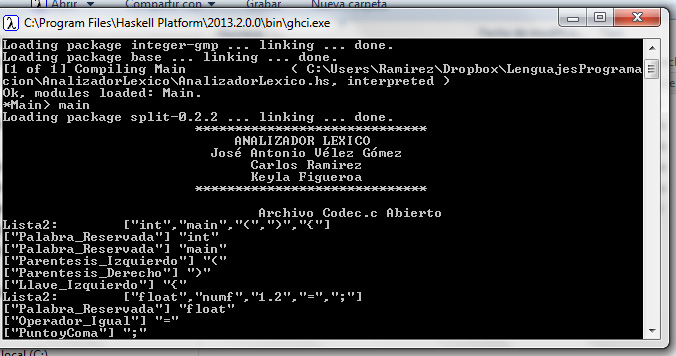
\includegraphics[width=.70\textwidth]{./imagenes/analizador.jpg}
\caption{haskell}
\label{haskell}
\end{center}
\end{figure}

\ \\ 
Haskell es un lenguaje de programaci\'on estandarizado multi-prop\'osito puramente funcional con sem\'anticas no estrictas y fuerte tipificaci\'on esta\'atica. Su nombre se debe al l\'ogico estadounidense Haskell Curry. En Haskell, una funci\'on es un ciudadano de primera clase del lenguaje de programaci\'on. Como lenguaje de programaci\'on funcional, el constructor de controles primario es la funci\'on. El lenguaje tiene sus origenes en las observaciones de Haskell Curry y sus descendientes intelectuales.
En los a�os 1980 se constituy\'o un comit\'e cuyo objetivo era crear un lenguaje funcional que reuniera las caracteristicas de los m\'ultiples lenguajes funcionales de la \'epoca, el m\'as notable Miranda, y resolviera la confusi\'on creada por la proliferaci\'on de los mismos.
El lenguaje evoluciona r\'apidamente con y  como los representantes actuales del est\'andar de facto. El \'ultimo est\'andar semi-oficial es Haskell 98, con la intenci\'on de especificar una versi\'on minima y compatible del lenguaje como base para futuras extensiones y para fines educativos.
Las caracter\'\i{}sticas m\'as interesantes de Haskell incluyen el soporte para tipos de datos y funciones recursivas, listas, tuplas, guardas y calce de patrones. La combinaci�n de las mismas pueden resultar en algunas funciones casi triviales cuya versi\'on en lenguajes imperativos pueden llegar a resultar extremadamente tediosas de programar.\ \\


\newpage
\section{GitHub:}
\begin{figure}[htbp]
\begin{center}

\includegraphics[width=.70\textwidth]{./imagenes/github_logo.jpg}
\caption{git}
\label{git}
\end{center}
\end{figure}

\ \\ 
GitHub es una forja para alojar proyectos utilizando el sistema de control de versiones Git. Utiliza el framework Ruby on Rails por GitHub, Inc. (anteriormente conocida como Logical Awesome).
Desde enero de 2010, GitHub opera bajo el nombre de GitHub, Inc.
El c\'odigo se almacena de forma publica, aunque tambi�n se puede hacer de forma privada, creando una cuenta de pago.
\ \\


\newpage
\section{Objetivos:}
\ \\ 
Crear una Analizador L\'exico en Haskell.
\ \\ 
Entender el funcionamiento de un Analizador l\'exico en un lenguaje de programaci\'on.
\ \\ 
Aprovechar Haskell como herramienta de desarrollo por su lenguaje funcional.
\ \\ 
Implementar nuestro Analizador haciendo uso de m\'etodos recursivos
\ \\ 
Utilizar GIT como herramienta de control de versionamiento.
\ \\ 

\section{Desarrollo:}
\ \\ 
El desarrollo de este tercer proyecto se realiz\'o entre tres integrantes del grupo, empezando por crear la funci\'on que nos permita cargar un archivo con nuestro c\'odigo c, entre otros archivos como la lista de identificadores, separadores y palabras reservadas.

El trabajo fue dividido entre los tres integrantes del grupo,  en este proyecto se incorpor\'o al grupo a Keyla Figueroa. 

La funcionalidad fue dividida entre Carlos Ram\'\i{}rez, Keyla Figueroa y Jos� V\'elez.

En este proyecto como es desarrollado en un Lenguaje funcional, se colabor\'o mutuamente en la implementaci\'on de nuestro Analizador L\'exico, investigando de diferentes fuentes el funcionamiento, formas de implementar mediante recursi\'on el an\'alisis del c\'odigo para encontrar los lexemes y clasificarlos por tokens.
El funcionamiento de nuestro analizador b\'asicamente consiste en leer nuestro archivo de c\'odigo fuente de C, y primero que todo limpiarlo de espacios y saltos de lineas, para un mejor an\'alisis del mismo por funciones split.
Luego se procedi\'o a cargar la lista de identificadores, palabras reservadas y separadores desde archivos distintos para proceder a verificar si existen en el c\'odigo C para empezar a clasificarlos por medio de tokens.
Luego se procedi\'o a identificar variables, n\'umeros y cadenas de caracteres dentro de nuestro c\'odigo C.
Para finalmente proceder a mostrar una lista de tuplas con los lexemes y sus respectivos tokens.
\ \\

\newpage
\section{Conclusiones:}
\ \\ 
La experiencia en Haskell, como herramienta de trabajo fue realmente algo novedoso por su lenguaje funcional, y como nos conlleva a pensar en soluciones de manera recursiva para un aprovechamiento de la herramienta, aparte de la no existencia de variables toda la experiencia en otros lenguajes no nos ayud\'o mucho para el desarrollo de este proyecto porque era una manera totalmente de programar, una perspectiva nueva.
Las ventajas de Haskell es su potencial con funciones recursivas y que incluye el soporte de tipos de datos junto al manejo de listas, tuplas fue una herramienta de gran utilidad para implementar nuestro Analizador L\'exico.
Se cumpli\'o con los objetivos planteados se us\'o Haskell como herramienta de desarrollo y entendimos el funcionamiento de un Analizador L\'exico.
\section{Referencias:}
\ \\ 

	http://aprendehaskell.es/

\ \\ 

	http://www.lcc.uma.es/~blas/pfHaskell/gentle/
\ \\ 

	http://www.haskell.org/haskellwiki/Tutorials
	
\ \\ 

	http://www.haskell.org/tutorial/
	
\ \\
\newpage